\chapter{Linear Regression, Ordinary Least Squares (OLS)}
\label{ch-linear-reg}
Wikipedia articles
\begin{enumerate}
\item
Linear Regression (LR)
\begin{itemize}
\item
linear regression, Ref.\cite{wiki-lr}
\item
 simple linear regression, Ref.\cite{wiki-slr}
\item
errors in variable, Ref.\cite{wiki-errors-in-iv}

\end{itemize}
\item
Least squares (LS)
\begin{itemize}
\item
least squares, Ref.\cite{wiki-lsquares}
\item
ordinary least squares (OLS), Ref.\cite{wiki-ols}
\end{itemize}
\end{enumerate}


Some nomenclature: In LR, the
data consists of
{\bf independent x-variables} $x^\s_1,
 x^\s_2, \ldots x^\s_n$
and a {\bf dependent y-variable} $y^\s$.
We find a linear fit $\haty^\s =
\beta_0 + \sum_{i=1}^n \beta_i x^\s_i$
to the data.
$\haty^\s$ is called the {\bf estimate}
of $y^\s$.
 The coefficients $\beta_0, \beta_i$
are called {\bf regression coefficients}.
$y^\s-\haty^\s=\eps^\s$
are called  the {\bf residuals}.
$\cale =\sum_\s (\eps^\s)^2$
is called the {\bf error or cost}. We choose the
regression coefficients
so as to minimize the error.

Below, we consider two types of LR:

\begin{enumerate}
\item
LR
in which the independent x-variables are non-random.
\item
LR
in which the independent x-variables are random
and i.i.d.
\end{enumerate}

The  term OLS
is often used to refer to LR
of type 1.



For LR of type 2,
there is randomness in $y$
coming from the randomness in $x$
and in the residuals.
For LR of type 1,
there  is randomness in $y$
too, but
it comes
from the residuals
only.

Once one assumes that certain
variables are random, a
\qt{model} (i.e., a bnet,
with probabilities expressed as TPMs)
 must be
specified.


\section{LR, assuming
$x^\s$ are non-random}

Let

$\s\in\{0, 1, 2, \ldots, nsam-1\}$ : sample index

$i_0\in\{0, 1, 2, \ldots, n\}$ :
index that can assume values 0 to $n$

$i\in\{1, 2, \ldots, n\}$ :
index that can assume values 1 to $n$.
$i$ is never equal to 0.


$y_\s\in \RR$: dependent y-variables

$x_{\s i}\in \RR$: independent x-variables

$\eps_\s\in \RR$: residuals

$\beta_0, \beta_i\in \RR$:
regression coefficients


\beq
y_\s= \beta_0 +
\sum_{i=1}^{n} x_{\s i}\beta_{i} + \eps_\s
\label{eq-LR-start}
\eeq

If we define
\beq
x_{\s 0}=1
\;
\eeq
for all $\s$, then

\beq
y_\s=
\sum_{i_0=0}^{n} x_{\s i_0}\beta_{i_0} + \eps_\s
\;.
\eeq
If $y$ and $\eps$ are $nsam$ dimensional
 column vectors and $\beta$
is an $n+1$ dimensional column vector,
and $X$ is an $nsam\times (n+1)$ matrix,
then we can write the previous equation in matrix
form as:


\beq
y=X\beta+\eps
\;.
\eeq

\subsection{Derivation of LR
 From Minimization of Error}

Let $W=[W_{\s, \s'}]$
be a symmetric matrix with non-negative
diagonal elements $W_{\s,\s}\geq 0$ for all $\s$.
$W$ is called the {\bf weight matrix}.
The following claim
describes the method of
{\bf Weighted LR}
when $W\neq 1$
and of simple LR  when $W=1$.
\begin{claim}
Assume the
Einstein summation convention; i.e.,
implicit sum over
repeated indices.
The
 error function $\cale$ given by

\beq
\cale=
\underbrace{(y_{\s}-X_{\s, j_0}\beta_{j_0})}
_{\text{residual $\eps_\s$}}
W_{\s, \s'}
\underbrace{(y_{\s'}-X_{\s', k_0}
\beta_{k_0})}_{\eps_{\s'}}
\;,
\eeq
is minimized
over $\beta_{k_0}$ for all $k_0
\in\{0,1,\ldots,n\}$,
if $\beta_{k_0}$ is given by:

\beq
\HAT{\beta}= (X^T W X)^{-1} X^T W y
\;.
\label{eq-betahat-non-ran-w}
\eeq
When $W=1$,

\beq
\HAT{\beta}= 
\underbrace{(X^T X)^{-1} X^T}_
{\partial_X} y
\;.
\label{eq-betahat-non-ran}
\eeq

\end{claim}
\proof

At the minimum of $\cale$,
the variation $\delta\cale$
 must vanish:
\beq
0=\delta \cale=
-2 X_{\s j_0}(\delta \beta_{j_0})
W_{\s, \s'}(y_{\s'}
-X_{\s' k_0}
\beta_{k_0})
\;.
\eeq
Thus,

\beq
X^T W y - X^T W X\beta=0
\eeq
which
implies Eq.(\ref{eq-betahat-non-ran-w}).
\qed

\subsection{Geometry of LR
with non-random $x^\s$.}

Recall that

\beq
y=X\beta+\eps
\;.
\eeq


Define the {\bf projection matrices}

\beq
I_X=X
\underbrace{(X^TX)^{-1}X^T}_{\partial_X}
\;,\;\;A_X=1-I_X
\eeq
A square matrix $M$
is symmetric if $M^T=M$
and is idempotent if $M^2=M$.
$I_X$ is symmetric
and idempotent
and so is $A_X$.
Note that $I_X$ and $A_X$
also satisfy:

\beq
A_XI_X=I_XA_X=0
\eeq
and

\beq
I_X X=X\;,\;\; A_X X=0
\;.
\eeq
$I_X$ acts as the identity on $X$, and
$A_X$ annihilates $X$.

One has

\beq
X^T(y-\eps)=X^T X\beta
\eeq
Hence

\beq
\beta=
(X^TX)^{-1}X^T(y-\eps)
\;.
\eeq


Define

\begin{subequations}
\beq \boxed{
\HAT{\beta}=
\underbrace{(X^TX)^{-1}X^T}_{\partial_X} \;y
\;,
}
\label{eq-beta-nonrandom-lin-reg}
\eeq



\beq
\HAT{y}=
X\HAT{\beta}= I_X y
\;,
\eeq
and

\beq
\HAT{\eps}=
y-X\HAT{\beta}=
y-\HAT{y}=(1-I_X)y=A_X y
\;.
\eeq
\end{subequations}
$I_X$ is sometimes  called the {\bf hat matrix},
because it gives $y$ a hat.

Given any function $f=f(y,X,\eps)$
and a scalar factor $\xi\in \RR$,
suppose
$f(\xi y, \xi X, \xi\eps)=\xi^\calo f(y,X,\eps)$.
Then we will say that $f(\cdot)$
is of {\bf order $\calo$ under scaling}.
Note that $\{\HAT{y},
 \HAT{\eps}\}$
are all of order 1 under scaling,
$\{\beta, \HAT{\beta}, I_X, A_X\}$
are all of order 0 under scaling,
and $\partial_X$ is of order $-1$ under scaling.
Thus, each curve-fit (i.e., symbol
with a hat)
scales the same way as its estimand (i.e., same
symbol
without a hat). Furthermore,
$\beta$, its curve-fit $\HAT{\beta}$, and
the projection matrices $I_X, A_X$
are invariant ($\calo=0$) under scaling.



Note that $y$
can be expressed as
a sum of 2 orthogonal estimates:



\beq
y= \underbrace{\HAT{y}}_{I_X y} +
\underbrace{\HAT{\eps}}_{A_X y}
\;.
\eeq
Fig.\ref{fig-lin-reg-vecs}
shows triangles representing
$y=X\beta+\eps$ and $y=\HAT{y}+\HAT{\eps}$.


\begin{figure}[h!]
\centering
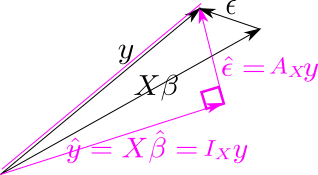
\includegraphics[width=2in]
{linear-reg/lin-reg-vecs.png}
\caption{Triangles
representing
$y=X\beta+\eps$ and $y=\HAT{y}+\HAT{\eps}$.}
\label{fig-lin-reg-vecs}
\end{figure}

\subsection{LR Goodness of Fit, $R^2$}

Assume $X$ and $\beta$ are not random.
This makes $\rvy=X\beta +\rveps$ and $\ul{\HAT{\beta}}=
\partial_X\rvy
$
random.

\begin{enumerate}
\item
First assume that the components of $\eps$
are random with zero mean:

\beq
E[\rveps]=\av{\rveps}=0
\eeq


One finds that

\begin{subequations}
\beq
\left\{
\begin{array}{l}
\av{\rvy}=X\beta
\\
\av{\HAT{\rvy}}=I_X
\underbrace{\av{\rvy}}_{X\beta}
=\av{\rvy}
\end{array}
\right.
\eeq

\beq
\left\{
\begin{array}{l}
\av{\rveps}=0
\\
\av{\HAT{\rveps}}=A_X
\underbrace{\av{\rvy}}_{X\beta}
=0=\av{\rveps}
\end{array}
\right.
\eeq

\beq
\av{\ul{\HAT{\beta}}}=
\partial_X \rvy = \av{\partial_X (\rvy-\rveps)}=\av{\beta}=\beta
\eeq


\item So far, we have
assumed a zero mean value for $\eps$.
Next, assume
{\bf  \qt{homoscedasticity} (homo-spread)}\footnote{I
 find the word \qt{homoscedasticity}
unnecessarily long, cryptic
and easy to misspell so
I like to replace
it by \qt{homo-spread}.
The opposite
of \qt{homoscedasticity}
is \qt{heteroscedasticity},
which I like to replace with \qt{hetero-spread}.}, which
means that

\beq
\av{\rveps, \rveps^T}=\xi^2 I_{nsam}
\eeq
\end{subequations}
where
$\xi\geq 0$,  and
$I_{nsam}$ is the
$nsam\times nsam$ identity matrix.
It follows that

\begin{subequations}
\label{eq-lin-re-variances}

\beq
\left\{
\begin{array}{l}
\av{\rveps, \rveps^T}=\xi^2 I_{nsam}
\\
\av{\HAT{\rveps},
\HAT{\rveps}^T}=
A_X\av{\rvy, \rvy^T}A_X^T=\xi^2A_X
\end{array}
\right.
\label{eq-homo}
\eeq

\beq
\left\{
\begin{array}{l}
\av{\rvy, \rvy^T}=
\av{\rveps, \rveps^T}=
\xi^2 I_{nsam}
\\
\av{\HAT{\rvy},
\HAT{\rvy}^T}=
I_X\av{\rvy, \rvy^T}I_X^T=\xi^2I_X
\end{array}
\right.
\eeq
and

\beq
\av{\HAT{\ul{\beta}},
\HAT{\ul{\beta}}^T}=
\partial_X\av{\rvy, \rvy^T}\partial_X^T=\xi^2 (X^TX)^{-1}
\;.
\eeq
\end{subequations}
\end{enumerate}
\hrule

For any random column vector $\rva$,
let

\beq
\norm{\rva}^2= \rva^T\rva=\tr(\rva\rva^T)
\eeq
Hence

\beq
\av{\norm{\rva-\av{\rva}}^2}=
\tr\av{\rva, \rva^T}
\;.
\eeq

Define the following sums of squares (SS):

\begin{subequations}
\label{eq-lin-reg-ss}
\beq
SS_{\rvy}=\av{\norm{\rvy-\av{\rvy}}^2}
=\tr\av{\rvy,\rvy^T}
\eeq

\beq
SS_{\HAT{\rvy}}=\av{\norm{\HAT{\rvy}-\av{\HAT{\rvy}}}^2}
=\tr\av{\HAT{\rvy},\HAT{\rvy}^T}
\eeq

\beq
SS_{res}=\av{\norm{\rvy-\HAT{\rvy}}^2}
=
\av{\norm{\ul{\HAT{\eps}}}^2}
=\tr\av{\ul{\HAT{\eps}},\ul{\HAT{\eps}}^T}
\eeq
\end{subequations}

\begin{claim}
The following is true
even if homo-spread
is violated:


\beq
\underbrace{\tr\av{\rvy,\rvy^T} }_{SS_\rvy}
=
\underbrace{\tr\av{\HAT{\rvy}, \HAT{\rvy}^T}}_{SS_{\HAT{\rvy}}}
+
\underbrace{\tr\av{\HAT{\rveps}, \HAT{\rveps}^T}}_{SS_{res}}
\eeq
This is like the Pythagorean Theorem
for the magenta right triangle
in Fig.\ref{fig-lin-reg-vecs}.
\end{claim}
\proof

From Eqs.\ref{eq-lin-re-variances}
and \ref{eq-lin-reg-ss},
we see that

\beq
SS_\rvy=\tr\av{\rvy,\rvy^T}
\eeq

\beq
SS_{\HAT{\rvy}}=\tr\av{\HAT{\rvy},\HAT{\rvy}^T}
=\tr\av{I_X\rvy, \rvy^T I_X^T}
=\tr\av{I_X\rvy, \rvy^T}
\eeq

\beq
SS_{res}=\tr\av{\HAT{\rveps}, \HAT{\rveps}^T}
=\tr\av{A_X\rvy, \rvy^TA_X^T}
=\tr\av{A_X\rvy, \rvy^T}
\eeq
Now use $I_X + A_X=1$.
\qed


The goodness of fit
for this model
is often measured using  the
{\bf coefficient of determination}
$R^2$. $R^2$  is defined by


\beq
R^2= 1 -\;\frac{SS_{res}}{SS_\rvy}=
\frac{SS_{\HAT{y}}}{SS_\rvy}
=
\frac{\tr \av{\HAT{\rvy},\HAT{\rvy}^T}}
{ \tr \av{\rvy,\rvy^T}}
\label{eq-r-sq-ss}\eeq
If homo-spread holds, then
$R^2$ reduces to


\beq
R^2 =\frac{\tr\; I_X}{nsam}
\;.
\eeq

See Fig.\ref{fig-pictorial-r2}
for a
pictorial explanation of $R^2$.
\begin{figure}[h!]
\centering
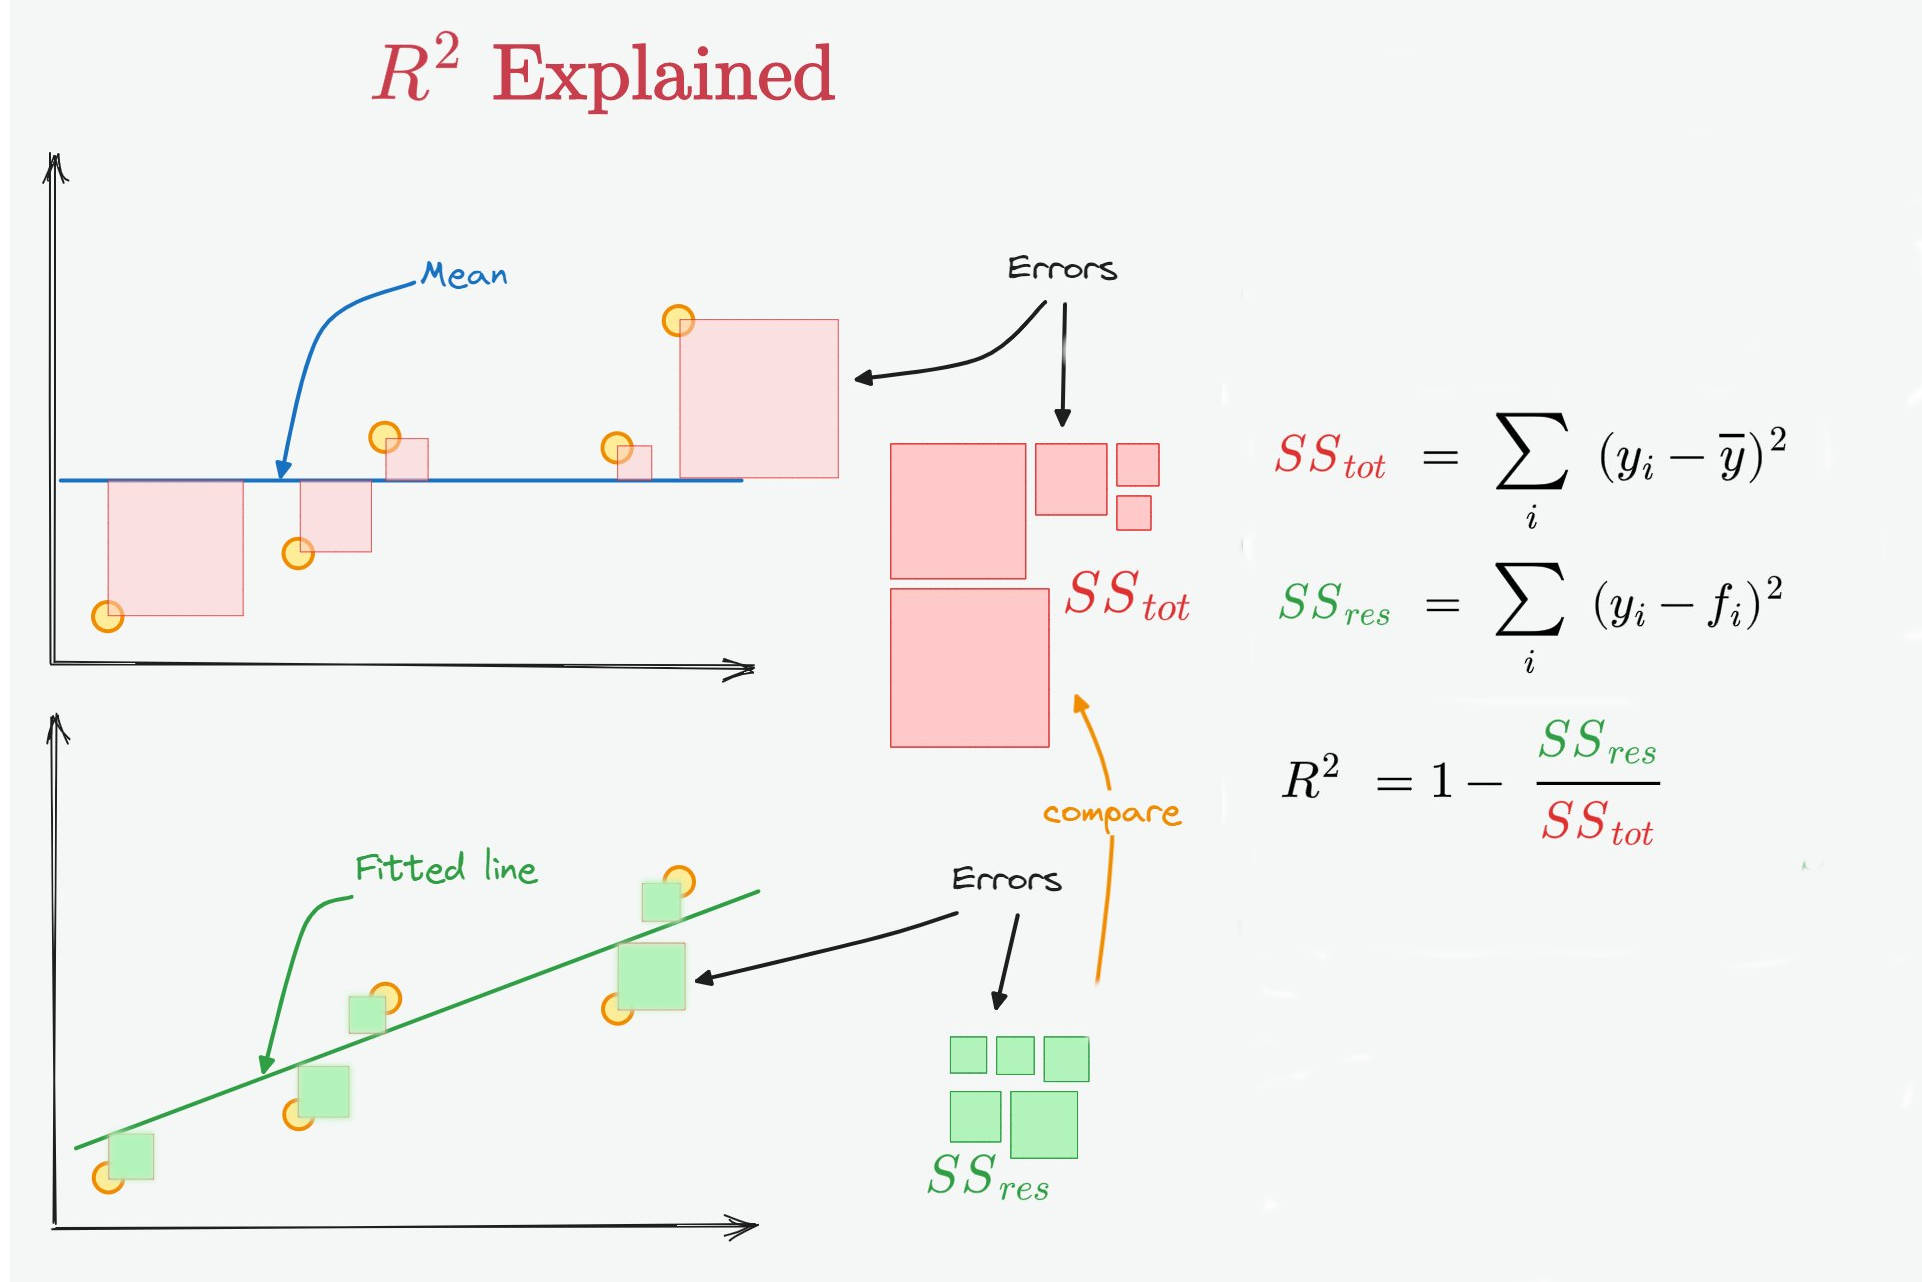
\includegraphics[width=6in]
{linear-reg/pictorial-r2.jpg}
\caption{Pictorial explanation of $R^2$.}
\label{fig-pictorial-r2}
\end{figure}



\section{LR, assuming
$x^\s$ are random}
Let

$i_0\in\{0, 1, 2, \ldots, n\}$ :
index that can assume values 0 to $n$

$i\in\{1, 2, \ldots, n\}$ :
index that can assume values 1 to $n$.
$i$ is never equal to 0.


$\rvy\in\RR$:  true value
of dependent y-variable

$\HAT{\rvy}\in\RR$: curve-fit
of dependent y-variable

$\ul{\eps}\in\RR$: residual



$\rvx_{i}\in \RR$: independent x-variables
for $i\in\{1,\ldots,n\}$

$\beta_0, \beta_i\in\RR$:
regression coefficients

\beqa
\HAT{\rvy}
&=&
\beta_0 +\sum_{j=1}^{n}
\beta_{j} \rvx_j
\\
&=&
\sum_{j_0=0}^{n}\beta_{j_0} \rvx_{j_0}
\;\;(\text{Assume $\rvx_0=1$.})
\eeqa

\beq
\rvy = \HAT{\rvy}+\ul{\eps}
\eeq

Fitting $y$
with a hyperplane
in the variables $x^n=(x_i)_{i=1}^n$
(i.e., finding
the best coefficients $\beta^n=(\beta_i)_{i=1}^n$)
is called {\bf regressing $y$ on $x^n$}.


\subsection{Transforming
from
non-random to
random $x^\s$ }

Define the following
population averages:


\beq
E_\s[x^\s]=
\frac{1}{nsam}
\sum_\s x^\s
\;,
\eeq

\beq
E_\s[x^\s y^\s]=
\frac{1}{nsam}
\sum_\s x^\s y^\s
\;,
\eeq

\beq
\av{x^\s,y^\s}_\s=
E_\s[x^\s y^\s]-E_\s[x^\s]E_\s[y^\s]
\;.
\eeq


\begin{claim}\label{cl-sigma-to-ran}
If the $x^\s$ are i.i.d. random
variables,

\beq
E_\s[x^\s] =\av{\rvx}
\;
\label{eq-exp-x}
\eeq
\beq
E_\s[x^\s y^\s]
=
\av{\rvx\rvy}
\label{eq-exp-xy}
\eeq

\beq
\av{x^\s,y^\s}_\s
=
\av{\rvx, \rvy}
\label{eq-exp-x--y}
\eeq
\end{claim}
\proof
\beqa
\frac{1}{nsam}
\sum_\s x^\s
&=&
\frac{1}{nsam}
\sum_{x\in S_\rvx}
x
\underbrace{
\sum_\s \indi(x^\s=x)}_
{N(x^\s=x)}
\\
&=&
\sum_{x}x\;P(x)
\\
&=&
\av{\rvx }
\eeqa

\beqa
\frac{1}{nsam}
\sum_\s x^\s y^\s
&=&
\frac{1}{nsam}
\sum_{x\in S_\rvx}
\sum_{y\in S_\rvy}
xy
\underbrace{
\sum_\s \indi(x^\s=x, y^\s=y)}_
{N(x^\s=x, y^\s=y)}
\\
&=&
\sum_{x,y}xy\;P(x,y)
\\
&=&
\av{\rvx \rvy}
\eeqa
Eq.(\ref{eq-exp-x--y})
follows from
Eq.(\ref{eq-exp-x}) and Eq.(\ref{eq-exp-xy}).
\qed

Recall that

\beq
Y_\s = \beta_0 +  \sum_{j=1}^n X_{\s,j}\beta_j + \eps_\s
\;.
\eeq

Assume
\beq
E_\s[X_{\s,k} \eps_\s]=E_\s[X_{\s,k}]
\underbrace{E_\s[ \eps_\s]}_{=0}=0
\;.
\eeq
Then we have

\beq
E_\s[X_{\s,k} Y_\s]=
E_\s[X_{\s,k}]\beta_0 + \sum_{j=1}^n
E_\s [X_{\s,k} X_{\s,j}] \beta_j +
\underbrace{E_\s[X_{\s,k} \eps_\s]}_{=0}
\label{eq-EXY}
\eeq
and

\beq
E_{\s'}[X_{\s',k}]E_\s[ Y_\s]=
E_{\s'}[X_{\s',k}]\beta_0 + \sum_{j=1}^n
E_{\s'} [X_{\s',k}] E_\s[ X_{\s,j}] \beta_j +
\underbrace{E_{\s'}[X_{\s',k}]  E_\s[ \eps_\s]}_{=0}
\label{eq-EX-EY}
\;.
\eeq
Subtracting
Eq.(\ref{eq-EX-EY}) from Eq.(\ref{eq-EXY}), we get

\beq
\av{X_{\s,k} ,Y_\s}_\s=
\sum_{j=1}^n
\av{X_{\s,k}, X_{\s,j}}_\s \beta_j
\label{eq-avX-comma-Y}
\;.
\eeq
Define the $n$ dimensional
covariance matrix $C$
by

\beq
C_{k,j}=\av{X_{\s,k}, X_{\s,j}}_\s
\:.
\eeq
Then Eq.(\ref{eq-avX-comma-Y}) implies

\beq
\beta_j =\sum_{k=1}^n
C^{-1}_{j,k} \av{X_{\s,k} ,Y_\s}_\s
\label{eq-beta_j-c-inv}
\eeq
for all $j=1,2,\ldots, n$.

If we assume that the $x^\s$ are i.i.d.,
then, by  virtue of Claim \ref{cl-sigma-to-ran},
the matrix $C$ tends to


\beq
C_{k,j}
\rarrow \av{\rvx_k, \rvx_j}
\eeq
and Eq.(\ref{eq-beta_j-c-inv})
implies

\beq
\beta_j = \sum_{k=1}^n C^{-1}_{j,k}\av{\rvx_k, \rvy}
\label{eq-beta-random-from-nonrandom}
\;.
\eeq

\subsection{LR with random $x^\s$,
expressed in derivative notation}

Recall our notation for {\it conditional} averages.(See sections
\ref{sec-notation-cov}, \ref{sec-cond-cov})
For any random
variables $\rvx, \rvy, \rva$, let

\beq
E_{|a}[\rvx]=\av{\rvx}^{|a}
\quad\text{(mean)}
\eeq

\beq
\av{\rvx, \rvy}^{|a}=
\av{\rvx\rvy}^{|a}
-
\av{\rvx}^{|a}\av{\rvy}^{|a}
\quad\text{(covariance)}
\eeq

\beq
\s_\rvx^{|a} =\sqrt{\av{\rvx, \rvx}^{|a}}
\quad \text{(standard deviation)}
\eeq

\beq
\rho_{\rvx, \rvy}^{|a}
=
\frac{\av{\rvx, \rvy}^{|a}}
{\s_\rvx^{|a} \s_\rvy^{|a}}
=
\left[
\frac{\av{\rvx, \rvy}}
{\s_\rvx \s_\rvy}
\right]^{|a}
\quad \text{(correlation)}
\eeq

\beq
\partial_\rvx^{|a}\rvy
=
\left[\pder{}{\rvx}\right]^{|a}\rvy
=
\frac{\av{\rvx,\rvy}^{|a}}
{\av{\rvx, \rvx}^{|a}}
=
\rho_{\rvx, \rvy}^{|a}\frac{
\s_\rvy^{|a}}
{\s_\rvx^{|a}}
=
\left[
\rho_{\rvx, \rvy}\frac{
\s_\rvy}
{\s_\rvx}\right]^{|a}
\quad\text{(partial derivative)}
\eeq
\qt{$|a$} means that the variable
$\rva$ is held fixed to $a$
when taking all averages.

Recall that

\beq
\rvy =
\underbrace{\beta_0 +\sum_{j=1}^{n}
\beta_{j} \rvx_j}_{\HAT{\rvy}}
+\ul{\eps}
\;.
\eeq


Assume

\beq
\av{\rveps}=0
\eeq
and
\beq
\av{\rvx_j, \ul{\eps}}=0
\eeq
for all $j$.

For $k=1, \ldots, n$,
\beq
\av{\rvx_k, \rvy}
=
\sum_{j=1}^{n}\beta_j\av{\rvx_k, \rvx_j}
\;.
\label{eq-beta-0-wrong}
\eeq
Define
the linear operator

\beq
\pder{\cdot}{\rva}=
\frac{\av{\rva, \cdot}}
{\av{\rva, \rva}}
\eeq
for any random variable $\rva$.
Then Eq.(\ref{eq-beta-0-wrong}),
after dividing both
of its sides by $\av{\rvx_k, \rvx_k}$,
can be written as

\beq
\pder{\rvy}{\rvx_k}=
\sum_{j=1}^n\beta_j\pder{\rvx_j}{\rvx_k}
\eeq
Let $\rvx^n$ and $\beta^n$ be
$n$-dimensional column vectors.
If we further define
the gradient

\beq
\nabla_{\rvx^n}\rvy
=\left[\pder{\rvy}{\rvx_1},
\pder{\rvy}{\rvx_2},
\ldots, \pder{\rvy}{\rvx_n}\right]^T
\eeq
and the Jacobian matrix
\beq
J_{j,k}=
\pder{\rvx_j}{\rvx_k}
\eeq
then

\beq
\nabla_{\rvx^n}\rvy=
J^T\beta^n
\eeq
so
\beq
\boxed{
\beta^n=
(J^T)^{-1}
\nabla_{\rvx^n}\rvy}
\label{eq-beta-j-nabla}
\eeq
Note that $J_{k,k}=1$ for all $k$.
Eq.(\ref{eq-beta-random-from-nonrandom})
and
Eq.(\ref{eq-beta-j-nabla})
are equivalent. Whereas the matrix
$C$ has the nice property
that it is symmetric,
the matrix $J$  has the nice
property that its diagonal
entries are 1.


Next, we will
write
 Eq.(\ref{eq-beta-j-nabla})
for the special cases
$n=1,2,3$,
where $n$ is the
number of independent x-variables $\rvx_j$.

\begin{enumerate}
\item $n=1$ ($\rvy$ fitted by a line)

\beq
\rvy = \beta_0 + \beta_1\rvx + \rveps
\eeq

Eq.(\ref{eq-beta-j-nabla}) becomes
\beq
\beta_1=\pder{\rvy}{\rvx}=
\frac{\av{\rvx,\rvy}}{\av{\rvx,\rvx}}
=
\rho_{\rvx,\rvy}
\frac{\s_\rvy}{\s_\rvx}
\eeq


\item $n=2$ ($\rvy$ fitted by a plane)


\beq
\rvy = \beta_0 + \beta_1 \rvx_1 + \beta_2 \rvx_2 +\rveps
\eeq
Eq.(\ref{eq-beta-j-nabla})
becomes\footnote{
Recall that if
$
M=
\left[
\begin{array}{cc}
a&b
\\
c&d
\end{array}
\right]
$
then
$
M^{-1}
=
\frac{1}{\det M}
\left[
\begin{array}{cc}
d&-b
\\
-c&a
\end{array}
\right]
$
}


\beqa
\left[
\begin{array}{c}
\beta_1
\\
\beta_2
\end{array}
\right]
&=&
(J^T)^{-1}
\left[
\begin{array}{c}
\partial_{\rvx_1}\rvy
\\
\partial_{\rvx_2}\rvy
\end{array}
\right]
\\
&=&
\frac{1}{\det J^T}
\left[
\begin{array}{cc}
J_{22}&-J_{21}
\\
-J_{12}&J_{11}
\end{array}
\right]
\left[
\begin{array}{c}
\partial_{\rvx_1}\rvy
\\
\partial_{\rvx_2}\rvy
\end{array}
\right]
\eeqa


Hence,
\beq
\beta_1
=
\frac{
J_{22}\partial_{\rvx_1}\rvy
-J_{21}\partial_{\rvx_2}\rvy
}
{
J_{11}J_{22}-J_{21}J_{12}
}=
\frac{
\partial_{\rvx_1}\rvy
-J_{21}\partial_{\rvx_2}\rvy
}
{
1-J_{21}J_{12}
}
\label{eq-beta-lr-plane}
\eeq
We can express
Eq.(\ref{eq-beta-lr-plane})
in terms of variances
and correlations as follows.


\beqa
\beta_1 &=&
\left[\frac{1}{\av{\rvx_1,\rvx_1}}\right]
\frac{\av{\rvx_1, \rvy}-
\av{\rvx_2, \rvx_1}
\av{\rvx_2, \rvy}
\av{\rvx_2, \rvx_2}^{-1}}
{1-\rho^2_{\rvx_1, \rvx_2}}
\\
&=&
\left[
\frac{1}{\s^2_{\rvx_1}}\right]
\frac{
\rho_{\rvx_1, \rvy}
\s_{\rvy}\s_{\rvx_1}
-\rho_{\rvx_1, \rvx_2}
\rho_{\rvx_2, \rvy}
\s_{\rvx_1}\s_\rvy
}{1-\rho^2_{\rvx_1, \rvx_2}}
\\
&=&
\left[
\frac{\s_\rvy}{\s_{\rvx_1}}\right]
\frac{
\rho_{\rvx_1, \rvy}
-\rho_{\rvx_1, \rvx_2}
\rho_{\rvx_2, \rvy}
}{1-\rho^2_{\rvx_1, \rvx_2}}
\label{eq-beta1-var-corr}
\eeqa
Eq.(\ref{eq-beta1-var-corr}) agrees with
the
value of $\beta_{YX, Z}$ in
Ref.\cite{pearl-lin-reg}
by Pearl,
if  we replace in Pearl's
formulae $X\rarrow \rvx_1$,
$Y\rarrow \rvy$, $Z\rarrow \rvx_2$.

Note that Eq.(\ref{eq-beta-lr-plane})
can also be written as


\beqa
\beta_1
&=&
\frac{
\partial_{\rvx_1}\rvy
-J_{21}\partial_{\rvx_2}\rvy
}
{
1-J_{21}J_{12}
}
\\
&=&
\partial_{\rvx_1}\rvy
+\underbrace{\frac{J_{21}J_{12}
\partial_{\rvx_1}-J_{21}
\partial_{\rvx_2}
}{1-J_{21}J_{12}}}
_{-A_{\rvx_1}}
\rvy
\eeqa
The linear operator $A_{\rvx_1}$
satisfies

\beq
A_{\rvx_1}(\rvx_1)=0
\quad\text{($A_{\rvx_1}$
annihilates $\rvx_1$)}
\eeq
and
\beq
A_{\rvx_1}(\rvx_2)=
J_{21}=
\partial_{\rvx_1}\rvx_2
\eeq
Therefore

\beq
A_{\rvx_1} = \partial^{|x_1}_{\rvx_1}
\eeq
and

\beq
\beta_1=
\partial_{\rvx_1}\rvy
-\partial_{\rvx_1}^{|x_1}\rvy
\eeq
If we define

\beq
I_{\rvx_1}=1-A_{\rvx_1}
\eeq
then

\beq
\beta_1 = \partial_{\rvx_1}
(I_{\rvx_1}\rvy)
\eeq

\item $n=3$ ($\rvy$ fitted by a volume)

\begin{figure}[h!]
$$
\xymatrix{
\rvx_1\ar[dd]\ar[rd]
\ar@/^1pc/[rrd]^{\beta_1}
&&\rveps\ar[d]
\\
&\rvx_2\ar[r]^{\beta_2}&\rvy
\\
\rvx_3\ar[ur]
\ar@/_1pc/[rru]_{\beta_3}
}
$$
\caption{Bnet for Linear Regression
of $\rvy$
with a 3 dimensional feature
vector $\rvx=(\rvx_1, \rvx_2, \rvx_3)$.
$\av{\rvx_j, \rveps}=0$ because
the path from $\rvx_j$
to $\rveps$ is blocked by a
collider node.
Note that even though node $\rvy$
is deterministic, nodes $\rvx_j$ may
be probabilistic. Hence, this is only
a partial LDEN
(LDEN are
discussed in Chapter \ref{ch-linear-sys})
}
\label{fig-LR-3x}
\end{figure}


\beq
\rvx^3 = [\rvx_1, \rvx_2, \rvx_3]^T
\eeq

\beq
\beta^3= [\beta_1,\beta_2, \beta_3]^T
\eeq

\beq
\rvy = [\beta^3]^T\rvx^3 + \rveps
\eeq

\beq
J_{i,j} =
\pder{\rvx_i}{\rvx_j}
\eeq

\beq
\beta^3=
(J^T)^{-1}\nabla_{\rvx^3}\rvy
\eeq

\beq
J^T
=
\left[
\begin{array}{ccc}
1&a_{12}&a_{13}\\
a_{21}&1&a_{23}\\
a_{31}&a_{32}&1
\end{array}
\right]=A
\eeq

\beq
a_{i,j}=
\pder{\rvx_j}{\rvx_i}
\eeq

Using Figs.\ref{fig-3dim-matrix}
and \ref{fig-3dim-matrix-inv}, we get

\begin{align}
\beta_1&=
\frac{1}{\det A}
\left(
\det{\left[
\begin{array}{cc}
1&a_{23}
\\
a_{32}&1
\end{array}
\right]}\partial_{\rvx_1}\rvy
+
\det{\left[
\begin{array}{cc}
a_{13}&a_{12}
\\
1&a_{32}
\end{array}
\right]}\partial_{\rvx_2}\rvy
+
\det{\left[
\begin{array}{cc}
a_{12}&a_{13}
\\
1&a_{23}
\end{array}
\right]}\partial_{\rvx_3}\rvy
\right)
\end{align}

\begin{figure}[h!]
\centering
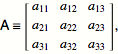
\includegraphics[width=1.5in]
{linear-reg/3d-matrix.png}
\caption{Arbitrary 3 dimensional matrix $A$}
\label{fig-3dim-matrix}
\end{figure}


\begin{figure}[h!]
\centering
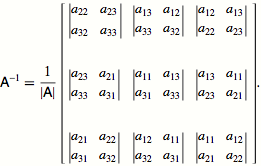
\includegraphics[width=3.5in]
{linear-reg/3d-matrix-inv.png}
\caption{Inverse of the 3 dimensional matrix $A$
given by Fig.\ref{fig-3dim-matrix}.}
\label{fig-3dim-matrix-inv}
\end{figure}






\end{enumerate}







\subsection{Regression on residuals
 of $y$}

Recall that

\beq
\rvy = \beta_0 + \sum_{j=1}^n \rvx_j \beta_j + \ul{\eps}
\;.
\eeq
Therefore,

\beqa
\av{\rvx_i, \rvy}
&=&
\sum_{j=1}^n \av{\rvx_i, \rvx_j}\beta_j
\\
&=&
 \av{\rvx_i, \rvx_i}\beta_i
+
\sum_{j=1}^n
\indi(j\neq i)
 \av{\rvx_i, \rvx_j}\beta_j
\;.
\eeqa
Hence,

\beq
\beta_i
=
\frac{\av{\rvx_i, \rvy}}
{\av{\rvx_i, \rvx_i}}
-\sum_{j=1}^n
\indi(j\neq i)
\frac{ \av{\rvx_i, \rvx_j}}
{\av{\rvx_i, \rvx_i}}
\beta_j
\;.
\label{eq-beta-i-non-deriv}
\eeq

Eq.(\ref{eq-beta-i-non-deriv})
can be expressed
in derivative notation as:

\beq
\beta_i
=
\pder{\rvy}
{\rvx_i}
-\sum_{j=1}^n\indi(j\neq i)
\pder{\rvx_j}
{\rvx_i}
\beta_j
\label{eq-beta-i-deriv}
\eeq
Note that,
because of the
linearity of the derivative operator,
Eq.(\ref{eq-beta-i-deriv})
implies:

\beqa
\beta_i&=&
\pder{}
{\rvx_i}
\left(\rvy
-
\underbrace{\sum_{j=1}^n
\indi(j\neq i)\rvx_j \beta_j
}_{\rvy-\rvx_i\beta_i-\beta_0-\rveps}
\right)
\\
&=&
\left[\partial_{\rvx_i}
-
\partial^{|x_i}_{\rvx_i}\right]\rvy
\label{eq-beta-i-2-steps}
\;.
\eeqa

Eq.(\ref{eq-beta-i-2-steps})
implies that if 
we know $(\HAT{\beta}_j)_{j\in \{1,2,
\ldots, n\}- \{ i\}}$,
we can regress
the residual
$\rvy
-\sum_{j\neq i} \rvx_j\HAT{\beta}_j$ on 
$x_i$, to get an
estimate of $\HAT{\beta}_i$.
For example, in the case $n=2$,
if we know $\HAT{\beta}_1$,
we can regress
the residual 
$\rvy-\rvx_1\HAT{\beta}_1$
on $\rvx_2$ to get an estimate
of $\HAT{\beta}_2$.




\subsection{$R^2$ with random $x^\sigma$}

Recall that

\beq
\rvy =
\underbrace{\beta_0 +\sum_{j=1}^{n}
\beta_{j} \rvx_j}_{\HAT{\rvy}}
+\ul{\eps}
\;.
\eeq


Assume

\beq
\av{\rveps}=0
\eeq
and
\beq
\av{\rvx_j, \ul{\eps}}=0
\eeq
for all $j$.

\beq
\HAT{\rvy} = \rvy -\rveps
\eeq

\beqa
\av{\HAT{\rvy}, \HAT{\rvy}}
&=&
\av{\HAT{\rvy}, \rvy-\rveps}
\\
&=&
\av{\HAT{\rvy}, \rvy}
\label{eq-cov-y-yhat}
\eeqa

\beqa
\av{\rvy, \rvy}
&=&
\av{\HAT{\rvy}-\eps,
\HAT{\rvy}-\eps}
\\
&=&
\av{\HAT{\rvy}, \HAT{\rvy}}
+
\av{\rveps, \rveps}
\label{eq-yvar-as-sum}
\eeqa

The goodness of fit measure $R^2$
for this model
is defined by
\beq
R^2_{{\rvy}\sim \HAT{\rvy}}
=
\frac{\av{\HAT{\rvy}, \HAT{\rvy}} }
{\av{{\rvy}, {\rvy}}}
=
1 - \frac{\av{\rveps, \rveps} }
{\av{{\rvy}, {\rvy}}}
\eeq
where we are using Eq.(\ref{eq-yvar-as-sum}).
By Eq.(\ref{eq-cov-y-yhat}), we
also have
\beq
R^2_{{\rvy}\sim \HAT{\rvy}}
=
\frac{\av{{\rvy}, \HAT{\rvy}}}
{\av{{\rvy},{\rvy}}}
=
\pder{\HAT{\rvy}}{\rvy}=
\rho_{\rvy, \HAT{\rvy}}
\frac{\s_{\HAT{\rvy}}}
{\s_\rvy}
\eeq

\beq
R^2_{{\rvy}\sim \HAT{\rvy}}
R^2_{\HAT{\rvy}\sim \rvy}=
\rho^2_{\rvy, \HAT{\rvy}}
\eeq




\section{Logistic Regression (LoR)}

Suppose
$x_\s\in \RR^n$,
$y_\s\in \RR$,
and $\Sigma$
is a population
of individuals $\s$.
In general,
a {\bf regression}
is when
we curve-fit a dataset
$\{(x_\s, y_\s):\s\in\Sigma\}$
with a function
$\haty=f(x)$.
In {\bf Linear
Regression (LR)},
which we
discussed earlier,
$f(x)$ is a hyperplane
in $x$.
On the other hand,
in {\bf Logistic Regression (LoR)},
$y_\s\in[0,1]$ and
$f(x)$ is the sigmoid of
a hyperplane in $x$.



More specifically, for LR
we have
Eq.(\ref{eq-LR-start})
which reads as follows:

\beq
y_\s=
\underbrace{
\beta_0 +
\sum_{i=1}^{n} x_{\s i}\beta_{i}
}_{\haty_\s}+ \eps_\s
\quad\text{(LR)}\;.
\eeq
For LoR, we have instead

\beq
p_\s=
\smoid\left(
\beta_0 +
\sum_{i=1}^{n} x_{\s i}\beta_{i} + \eps_\s
\right)
\quad\text{(LoR)}\;,
\eeq
or, equivalently,


\beq
\underbrace{\lodds(p_\s)}
_{\ln \frac{p_\s}{1-p_\s}}=
\underbrace{
\beta_0 +
\sum_{i=1}^{n} x_{\s i}\beta_{i}
}_{\haty_\s} + \eps_\s
\quad\text{(LoR)}\;,
\eeq
where we have used the fact that
$\lodds()$
is the inverse function of $\smoid()$.
Hence, an LoR
fit can be calculated by
collecting a dataset
$\{(x_\s, p_\s):\s\in\Sigma\}$,
transforming that
dataset to the dataset
$\{(x_\s,\lodds( p_\s)):\s\in\Sigma\}$,
and fitting the latter dataset
with a hyperplane.
Let $P(\rvY_\s=1)=p_\s\in [0,1]$.
LoR can be used
for binary
classification
if we define the
binary class
variable $c_\s\in \bool$ by

\beq
c_\s =\indi(P(\rvY_\s=1)>\alp)
\eeq
for some $0<\alp<1$.